\section{Motivation}\label{sec:background}\label{sec:motivating}

%\aditya{is this a motivation for why we need guardrails or for our design of guardrails? accordingly, make the section title precise}
%\sujay{I have attempted to make the first part about why we need guardrails. And the second part about design of guardrails.}

Traditionally, OS policies are designed to perform well across a broad range of workloads and hardware configurations. However, growing workload diversity and hardware heterogeneity have driven increasing interest in designing policies tailored to specific deployment contexts to achieve better performance.
Recent research has focused on enabling customization of OS policies using eBPF~\cite{sched-ext,cache-ext-sosp25,pageflex2025}, tuning OS parameters per workload~\cite{tuning-pacmi25,agentic-tuning-ml4sys25}, and developing learned policies~\cite{heimdall-eurosys25,orca-sigcomm20,kml-tos23,kleio-hpdc19,linnos-osdi20}. More recently, researchers are leveraging AI agents to generate specialized heuristics~\cite{policysmith-hotnets25,glia-arxiv25,barbarians25,vulcan-arxiv25,agentic-os-ml4sys25}.
Whether traditional or specialized, all these policies share a common limitation: developers typically evaluate them on a limited set of benchmarks before deployment, with no mechanism to verify that the policy continues to meet its performance goals during runtime.

% Typically, OS policies are designed to achieve performance requirements such as increased throughput or reduced latency. Standard practice is to justify those requirements empirically using offline benchmarks. This statistical evidence is limited by the workloads and environments on which the policy was evaluated, and those assumptions have proven not to hold in in deployed systems. For instance, the LinnOS~\cite{linnos-osdi20} system predicts I/O latency from request and device features, trained on a specific class of devices; However, the latency accuracy degrades when deployed on faster devices~\cite{heimdall-eurosys25}.

\subsection{Brittle Assumptions in Modern OS Policies}

\begin{figure}[t]
    \centering
    \setlength{\belowcaptionskip}{-10pt}
    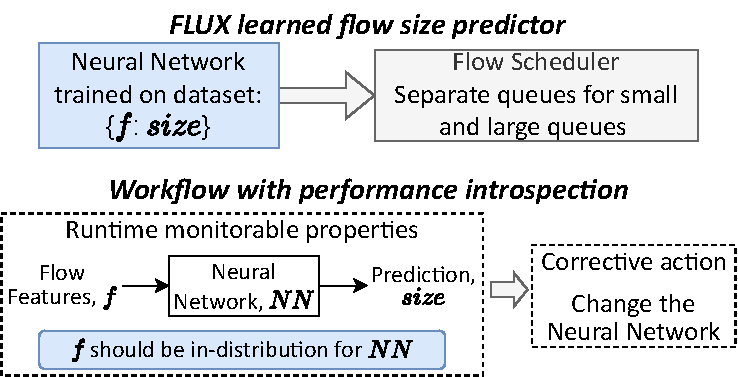
\includegraphics[width=0.7\columnwidth]{figures/Examples/FLUX-example.pdf}
    \caption{A common challenge: learned predictors care about good accuracy, but fixing performance degradations requires constant offline retraining. Instead, we propose run-time checks using observable proxies such as input-distribution checks.}
    \label{fig:flux-example}
\end{figure}

\begin{figure}[t]
    \centering
    
    \setlength{\belowcaptionskip}{-10pt}
    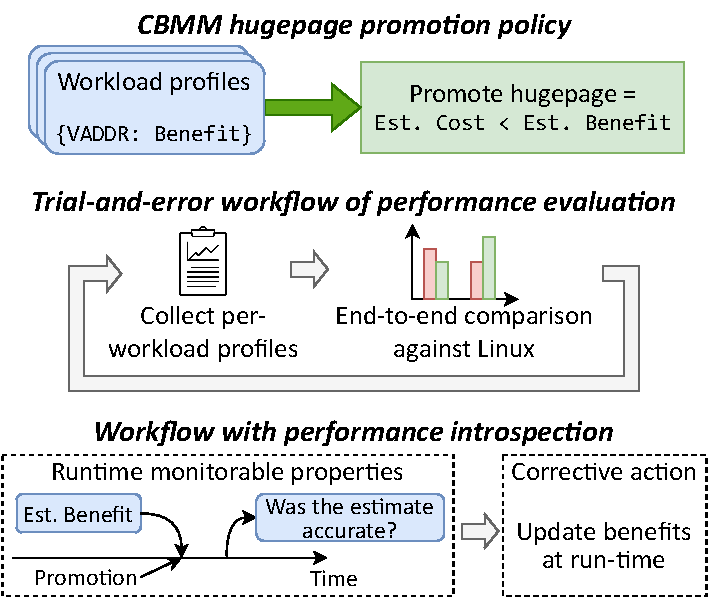
\includegraphics[width=0.7\columnwidth]{figures/Examples/CBMM-example.pdf}
    \caption{CBMM illustrates an additional challenge: the policy cares about correctness of promotion decisions, but any run-time check must rely on currently observable signals.}
    \label{fig:cbmm-example}
\end{figure}

We provide two examples to demonstrate how policies designed under certain assumptions or conditions can fail when those assumptions break at deployment time.

\noindent
{\it \textbf{Learned Flow Scheduling using FLUX.}}
% Learned predictors often perform well on in-distribution workloads but can degrade substantially under out-of-distribution ones.
Policies tuned or trained offline can silently degrade when deployment conditions or assumptions diverge from what they were built for.
Consider the FLUX learned flow scheduler~\cite{flux-nsdi19} (see \Cref{fig:flux-example}), which aims to reduce flow completion times. FLUX learns a model that predicts the completion time of a flow $f$ from a vector of run-time features $\vec v$, such as size and inter-arrival behavior, and uses these predictions to prioritize flows with smaller predicted completion times.
We observe that FLUX provides 75\% accuracy on large flows that match its training distribution, but degrades substantially (resulting in mere 21\% accuracy) on smaller flows that fall outside it. 
Unfortunately, the scheduler has no means to detect that the model has become unreliable and continues to use its predictions. 
% \sujay{@Divyanshu add numbers}

\noindent
{\it \textbf{Hugepage promotion in CBMM.}}
Even policies that are not learned can embed offline assumptions that silently break at deployment time. A concrete example arises in hugepage promotion.
Hugepages reduce TLB misses and address-translation overhead, but promoting them also incurs allocation and compaction costs and can increase memory bloat.
CBMM~\cite{cbmm-atc22} addresses this tradeoff by promoting a region only when an estimated promotion benefit exceeds an estimated promotion cost (see \Cref{fig:cbmm-example}), where the benefit estimates are profiled offline and the costs are derived from current system state. But, as workloads drift, those profiled benefit estimates may no longer reflect deployment-time behavior.

Such performance degradations are not uncommon -- they arise throughout the OS, from heuristic-based eviction policies for the page cache~\cite{cache-ext-sosp25} to learned I/O admission control for storage arrays~\cite{linnos-osdi20}.
In all of the above examples, the common practice for developers or infrastructure operators is to fall back on offline evaluation across a range of workloads (as shown in \Cref{fig:cbmm-example,fig:flux-example}), followed by manual inspection of end-to-end performance metrics.
This process is tedious, incomplete, and ultimately unsatisfactory: no finite offline evaluation can anticipate the diversity of executions encountered in deployment.

These examples motivate the need for a common framework for monitoring policy behavior at runtime and responding when they perform poorly. However, doing so requires overcoming fundamental challenges. % discussed below.

\subsection{Challenges with Runtime Monitoring}
The central challenge is determining what performance properties to monitor during runtime. Operators typically reason about high-level objectives such as tail latency, completion times, or eventual properties such as fairness. However, these metrics are not always observable within the OS.
A runtime monitoring system must therefore work with signals that the OS can observe, even when the operator's true objective lies outside the kernel's visibility. This raises another question: how can a local, kernel-observable property provide meaningful assurance about a high-level objective?

The CBMM example from \Cref{fig:cbmm-example} illustrates this tension concretely. The main objective of CBMM policy is that the promotion decisions should not degrade significantly relative to the decisions one would make using the true runtime benefits. Unfortunately, that objective is not directly observable at promotion time, because the true benefit of a promotion depends on future accesses.
What the OS can monitor, however, is whether stored benefit estimates follow the same order as recent accesses for different page regions.
This property is useful because, under the assumption that true runtime benefit is monotone with observed accesses, access ordering serves as a proxy for true-benefit ordering. If the estimated-benefits then match the access ordering, then the policy is more likely to preserve the intended comparison between benefit and cost at promotion time. Therefore, if the two orderings diverge, the stored profile is likely stale. A corrective action can then update the estimated benefits to restore this alignment, thereby helping preserve the quality of the resulting promotion decisions.


% While the performance objective is directly monitorable. In FLUX, the high-level objective of low flow completion times remains directly observable after the fact: once flows complete, the system can measure realized flow completion times and determine whether FLUX is continuing to deliver low average $\mathsf{FCT}$. If not, the system can revert to a safer alternative such as the default Linux scheduler.
% In many cases, it might not be possible to monitor a user's high-level objective within the OS kernel because it does not have access to it. While the performance objective may not itself what the OS can check at the point where it must act, but there is a run-time signal that allows it to infer \emph{something useful} about that objective. For instance, if the requirement is that queueing delay remain below a target $D$, the OS need not measure delay directly: in a FIFO queue with occupancy $q$ and service rate at least $\mu_{\min}$, the waiting time satisfies $W_q \leq q / \mu_{\min}$. Thus, enforcing $q \leq \mu_{\min} D$ is sufficient to ensure $W_q \leq D$. 

% \paragraph{Directly Observable Performance Objectives.}
% In some cases, the performance objective is directly monitorable. For example, if the requirement is that a subsystem maintain queue occupancy below a bound, say $\forall q.\;\mathsf{occupancy}(q) < N$, then the relevant quantity is available on the execution path, and the OS can monitor it directly and intervene when the bound is exceeded. 

% Returning to the FLUX example, its high-level objective, (based on $\mathsf{FCT}$s) however, remains directly observable after the fact: once flows complete, the system can measure realized flow completion times and determine whether FLUX is continuing to deliver low average $\mathsf{FCT}$. If not, the system can revert to a safer alternative such as the default Linux scheduler.


% \paragraph{Indirectly Observable Performance Objectives}
% However, in many important cases, 
% The same pattern appears in other familiar settings. In real-time scheduling, nonnegative slack implies deadline feasibility; in memory allocation, maintaining free-memory watermarks implies avoidance of reclaim-induced stalls. In all of these cases, the system monitors a signal that is not the objective itself, but that nevertheless provides a principled basis for intervention.


\subsection{Lessons for a New Framework}\label{subsec:lessons}

The examples above point to a common lesson: whether or not the ultimate performance objective is directly observable, one can often identify useful signals that indicate whether a policy is still operating in the regime for which it was designed. Unfortunately, today, such signals are rarely utilized. In many cases, OS policy designers do not attempt to detect regime shift at all; in other cases, they must handcraft monitoring and recovery logic that is tightly coupled to a particular policy and therefore difficult to reuse~\cite{linnos-osdi20,llama-asplos20,ingens-osdi16,sol-asplos22}.

The central thesis of this paper is that this should not be left to ad hoc mechanisms. Detecting when a policy has drifted out of its intended regime, and reacting appropriately when that happens, should be a first-class OS capability. The OS should provide a unified framework for specifying which signals matter, monitoring them at low overhead, and triggering corrective actions when needed. The framework proposed in this paper provides this capability through intuitive specifications and efficient in-kernel enforcement.

Another lesson from these examples is that identifying useful run-time signals is only part of the problem: those signals must ultimately connect back to some {\em higher-level performance objective}, such as promotion decisions being accurate for CBMM.
More broadly, such performance objectives may also require multiple runtime monitors, each capturing a different aspect of whether the policies are behaving as intended.
In such cases, simply reasoning about how a single runtime signal leads to the performance objective is not enough. The framework should additionally support compositional reasoning about how {\em collections} of local checks and repairs are \emph{jointly sufficient} to achieve the higher-level objective. 


% More broadly, the proposed framework is not limited to settings in which a single signal directly exposes a single failure mode. Many important objectives require multiple signals, each capturing a different aspect of whether the policy is behaving as intended. In such cases, no single guardrail is sufficient in isolation. Instead, different guardrails may need to monitor different signals and trigger different corrective actions, each addressing a distinct way in which the policy can drift out of its intended regime. To tackle this more challenging setting, our framework supports compositional reasoning about \emph{collections} of guardrails, making it possible to show that these local checks and repairs are \emph{jointly sufficient} to achieve a {\em higher-level performance objective}. 

% Taken together, these examples suggest a simple taxonomy: Some performance objectives are directly observable during execution; some are not observable within a run at all; and many of the most important ones are only indirectly observable through run-time signals that support a principled inference about the true objective. What is missing today is a systematic way to express which signals should be monitored, what corrective action should follow when they indicate a problem, and why those local checks are sufficient for the end-to-end property the designer actually cares about.l

% \subsection{The Observability Gap}

% In simple cases, the OS can directly check whether a subsystem is meeting its performance requirements. If the requirement is that a subsystem keep queue occupancy, run-queue length, or compaction overhead below a bound, the relevant quantities are already present on the execution path or in kernel-maintained counters, then the OS can monitor those quantities online, and can intervene when those bounds are exceeded. In such cases, the run-time check can coincide directly with the performance objective itself.

% On the opposite extreme, the OS wants to ensure that the policy is performing as intended, but cannot check the relevant performance condition directly. For instance, in SRTF scheduling, the OS wants to ensure that the scheduler is correctly prioritizing short jobs, because knowing how long a job will take requires knowledge of the future. The OS cannot preemptively check whether the scheduler is prioritizing short jobs. In this case, the only solution is post-hoc monitoring: the OS can check after the fact whether the scheduler's decisions were good, but it cannot know at decision time whether they will be. In such cases, the run-time is necessarily decoupled from the performance objective itself.

% However, many relevant cases fall somewhere in between, where there are runtime-observable signals that are directly related to the performance objective, but that do not directly measure it. For example, in CB 

% but it cannot know at dispatch time which jobs are actually short. In CBMM, the OS wants to ensure that hugepage promotions are paying off, but it cannot know at promotion time how future accesses will unfold. In learned scheduling, the OS wants to ensure that the model is making good predictions, but it cannot know at decision time how the flow will behave or how the queueing interactions will evolve.

% The OS must rely on surrogates that stand in for the true objective.
% The observability gap is the mismatch between the performance property the designer ultimately cares about and the evidence the OS can access at the time intervention is needed. Some performance properties can be checked directly during execution using kernel-visible quantities such as run-queue lengths, queue occupancies, allocator latency, or CPU time spent in a subsystem. Others cannot. Whether a hugepage promotion will pay off depends on future accesses; whether a learned scheduler made a good decision may depend on an outcome that arrives only later; whether a policy improved application throughput or tail latency may require external or counterfactual information.

% This distinction is fundamental because the OS can intervene only on the basis of what it can observe online. When the desired objective is directly monitorable, the run-time check can coincide with the objective itself or with a close operationalization of it. When it is not, the policy must rely on run-time surrogates that stand in for the hidden objective. Performance then depends not only on the policy logic, but also on whether those surrogates continue to track what the system actually cares about.

% This section develops that point. We first contrast cases in which the relevant performance condition is directly monitorable with cases in which it is not. We then show that the same observability gap appears across several OS subsystems. Finally, we use this gap to motivate performance introspection: a framework in which the run-time check, the corrective action, and the connection to the higher-level objective are all made explicit.

% \subsection{Directly Monitorable Performance Objectives}
% At one end are objectives that the OS can evaluate directly. For example, if memory compaction should not impose excessive overhead, the kernel can measure time spent in {\tt compact\_zone()} over recent windows and can disable or throttle hugepage promotion when that bound is exceeded. In such cases, the monitored condition is already close to the true objective. The check is local, online, and does not require prediction or oracle knowledge.



% CBMM~\cite{cbmm-atc22} chooses hugepage promotions by comparing estimated benefit against cost. Part of this decision problem is visible online: the current cost of promotion depends on quantities such as free or zeroed pages and on current compaction behavior. The key benefit term is not. The relevant quantity is the future reduction in address-translation cost obtained while the region remains promoted, and that quantity depends on accesses that have not yet occurred. The condition the designer ultimately cares about, namely that the system promote a region only when its future benefit exceeds its cost, is therefore not directly checkable at the time the decision is made. A run-time mechanism must instead monitor a surrogate, such as whether recent access behavior continues to preserve the ranking implied by the stored benefit estimates. When that surrogate fails, the system has evidence not that the objective itself was directly observed, but that the proxy used to approximate it has drifted out of alignment with the current execution.



% \subsection{Indirectly Monitorable Performance Objectives}

% % \subsection{A Pervasive Observability Gap}

% % This structure is not specific to CBMM or to learned scheduling. {\tt cache\_ext}~\cite{cache-ext-sosp25} shows that the best page-cache eviction heuristic varies across workloads. The objective is end-to-end hit rate or throughput, but the kernel must make online decisions using local signals such as recency, frequency, and observed reuse. Similarly, LinnOS~\cite{linnos-osdi20} predicts I/O latency from request and device features, yet Heimdall~\cite{heimdall-eurosys25} later shows that predictor accuracy can degrade on faster devices. At dispatch time, the system can inspect current request state, but it cannot yet know the true service time that would validate the prediction. Across memory management, caching, storage, and learned scheduling, the same mismatch recurs: the quantity the designer cares about is often global, delayed, or workload-dependent, whereas the quantity the OS can test online is local and immediate.

% % This is the setting in which deployment-time assumptions matter. Profiles, predictors, and tuned heuristics are not problematic merely because they are specialized. They are problematic because each of them compresses a hard-to-observe objective into a run-time surrogate. A workload shift, feature-distribution shift, or hardware change breaks precisely that correspondence. What fails is often neither functional correctness nor the existence of a policy decision, but the relationship between the signals observed online and the objective the policy was meant to optimize.

% \subsection{Why This Calls for Performance Introspection}

% The consequence is that performance introspection cannot be reduced to generic end-to-end monitoring. Collecting throughput numbers or tail latencies after the fact can reveal that performance regressed, but it does not tell the system what it can check online, when it should intervene, or which local condition has ceased to track the intended objective. A practical mechanism must instead work with conditions that are evaluable inside the OS during execution, cheap enough to monitor continuously, and informative enough to support action.

% When the desired objective is directly monitorable, the run-time condition may coincide with the objective itself or with a close operationalization of it. When the objective depends on future, external, or counterfactual information, the run-time condition is necessarily a proxy. In that case, the central design question is not only what the policy is trying to optimize, but also which observable condition best indicates that the policy is still operating in the regime for which it was designed. The corresponding response must likewise be executable online: update a parameter, switch to another installed policy, or fall back to a safer default.

% Performance introspection makes this structure explicit. It requires the designer to state which run-time condition will be monitored, what corrective action is available when that condition fails, and, when the condition is only a surrogate, why maintaining or restoring it supports the higher-level objective. This is the role of guardrails. The next section presents a framework for expressing such guardrails, while later sections formalize how local run-time checks can be related to the global performance objectives that motivated them in the first place.
